\documentclass[a4paper,12pt]{article}

\usepackage{setspace}
\usepackage{graphicx}
\usepackage{float}

\onehalfspacing
\boldmath

\newcommand{\vir}[1]{``#1''}

\begin{document}

\title{MSc Preliminary Project Report \\ \textbf{Design, Implementation and Testing of a Constructive Neural Network Algorithm}}
\author{Student: \textbf{Andrea Orru} (andrea.orru@kcl.ac.uk, ID: 1473018) \\ Supervisor: \textbf{Michael Spratling}}
\date{\today}
\maketitle

\section{Introduction}
	Artificial neural networks in their various incarnations have been successfully used to solve a very wide
	range of machine learning problems, thanks to their good representational capabilities \cite{sharma2010constructive}.
	
	Theoretically, a simple feed-forward neural network with a single hidden layer and a sufficient number of neurons in that layer is an universal approximator \cite{hornik1989multilayer}.
	In practice however, too small networks may be unable to adequately learn the problem, while overly large networks tend to overfit the training data \cite{parekh2000constructive}.
	
	The problem of determining the optimum neural network topology is thus very important. However, there are currently no efficient methods to choose \emph{a priori}
	the best network architecture for a given problem \cite{parekh2000constructive}.
	In real-world applications, trial-and-error and decisions based on previous knowledge about the problem are often the preferred approach. The chosen architecture
	has thus no guarantees to be the optimal one for the task \cite{parekh2000constructive}\cite{sharma2010constructive}.
	
	To solve this issue, solutions that involve learning both the weights of the synapses \emph{and} the network topology have been suggested \cite{parekh2000constructive}.
	One of the proposed answers is the class of algorithms of \emph{constructive neural networks}. The main idea behind them is to start from a minimal architecture and then add
	hidden layers, nodes and connections during training \cite{sharma2010constructive}.
	This provides the flexibility to explore the space of neural network topologies in a controlled, data-driven fashion.
	Furthermore, because small solutions are found first, this method has the potential to discover near-minimal networks that approximately match the complexity of the learning task \cite{parekh2000constructive}.
	
	For the purpose of this project we are interested in developing a constructive version of the \emph{Divisive Input Modulation} (DIM) learning algorithm.
	This algorithm has been developed to train a variation of \emph{negative feedback networks} and has proven to be very successful in the
	task of unsupervised learning of image components.
	The main feature of this class of networks is to implement competition between nodes, which is a way to enable them to be selective for different input stimuli.
	This is achieved by having inhibiting feedback connections from the output nodes to the input of those nodes \cite{spratling2009unsupervised}.
	
	An alternative but equivalent way of looking at this model is that the higher level of the network predicts the input it expects to receive via feedback connections;
	feedforward connections instead convey residual error between top-down prediction and bottom-up input \cite{spratling2008predictive}.
	
	Most notably, the \emph{non-linear PC/BC} (Predictive Coding as Biased Competition) model proposes a way to represent how biological visual cortex areas work
	by means of hierarchical neural networks: each neighbouring cortical region is a stage implemented as a layer of error-detecting nodes and a layer of competing predicting nodes, as previously explained.
	More interestingly, the outcome of the competiton is influenced both bottom-up by earlier stages \emph{and} top-down by higher levels of the stage chain \cite{spratling2008predictive}.
	
	The PC/BC model makes use of Divisive Input Modulation to extract elementary image components from both artificial and natural images.
	For natural images, components resembling Gabor functions are learnt in the first stage and neurons responsive to corners are learnt in the second stage.
	This closely resembles the behaviour shown by primary visual cortex (V1) and V2. Being the method unsupervised, this proves the biological soundness of the model \cite{spratling2012unsupervised}.
	
	The goal of the project is to develop a version of the DIM algorithm for PC/BC networks which learns a near-optimal topology alongside feedforward and feedback weights.
	Starting from a minimal structure, neurons can be added into the predictive layers if the error values do not converge. Different set of parameters and thresholds
	will be tested, and various approaches, such as whether to relearn all the weights from scratch after growing the network, will be experimented.
	Results will be continuously tested against standard unsupervised learning benchmarks such as the bars problem \cite{spratling2009unsupervised} and the squares problem \cite{spratling2012unsupervised}.
	
	The next section will provide additional details on the structure of the hierarchical neural network implementing the PC/BC model, on the DIM algorithm and on exhisting constructive neural network algorithms.
	I will show some ways in which those algorithms can be modified and applied to the proposed problem. In the end, a Gantt chart for the plan of the project development will also be provided.

\section{Background material}
	\subsection{Divisive Input Modulation}
		Divisive Input Modulation (DIM) is a novel neural network training algorithm designed for the unsupervised learning of image components.
		It is inspired by the observation that non-negative matrix factorisation (NMF) shares mathematical similarity with negative feedback neural networks.
		In particular, NMF can be seen as a divisory form of feedback inhibition. However, the main difference is that NMF operates in batch mode,
		while negative feedback neural network is an on-line algorithm. \cite{spratling2009unsupervised}
		
		Non-negative matrix factorisation is a method to find two non-negative factors $W^T$ and $Y$ of a non-negative matrix $X$, such that:
		$$X \approx W^T Y$$
		Since image components are non-negative, theoretically this is a suitable method to find parts-based decomposition of an images \cite{spratling2009unsupervised}.
		If $m$ is the size of the images, $n$ is the number of possible image components, and $p$ is the number of images in the training set, then:
		\begin{itemize}
			\item $X = [x_1, ..., x_p]$ is an $m \times p$ matrix, with each column containing the pixels of a training image.
			\item $W^T$ is an $m \times n$ matrix of weight values, with each column being a component (or basis vector) into which an image can be decomposed.
			\item $Y = [y_1, ..., y_p]$ is an $n \times\ p$ matrix, with each column describing the activation of each component in the corrisponding training image.
		\end{itemize}
		An individual training image can be reconstructed as $x_k \approx W^T y_k$. \cite{spratling2009unsupervised}
		There exists a number of algorithms to approximate the solutions for that equation. However, all of them operate on all the training data at once.
		
		In analogy to negative feedback networks, the term $E = X \oslash (W^T Y)$ which measures the residual error in the reconstruction of $X$, can be introduced.
		By performing the relevant substitutions and on the basis of some simplifying assumptions (detailed in \cite{spratling2009unsupervised}), the formulas can be rewritten
		and iterative rules for the vectors relative to a single training image (written in lowercase) can be derived:
		$$e = x \oslash (\epsilon + \hat{W}^T y)$$
		$$y \leftarrow (\epsilon + y) \otimes We$$
		$$W \leftarrow W \otimes (1 + \beta y (e^T - 1))$$
		Where $\hat{W}$ is a matrix representing the same synaptic weight values as $W$ but with rows normalised to have a maximum value of 1, and $\epsilon$
		is a small constant used to prevent division-by-zero errors. Following learning, weights are clipped at zero.
		\begin{figure}[H]
  			\centering
			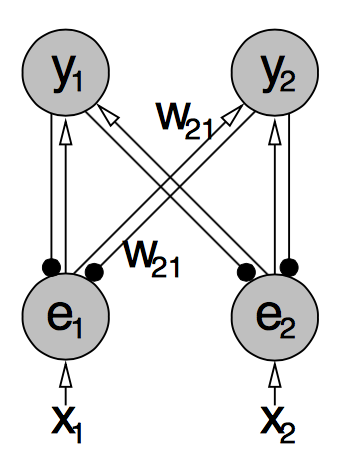
\includegraphics[scale=0.5]{nn}
			\caption{The structure of a simple neural network of the type used by Divisive Input Modulation \cite{spratling2009unsupervised}.}
		\end{figure}
		$e$ indicates the discrepancy between the top-down reconstruction of the input and the actual input; when it is equal to 1, the reconstruction is perfect and the weights
		stop changing as can be seen from the equation for $W$. By means of the same equation, if an error-detecting node is under-represented, the weights between it
		and active output nodes are increased, and vice-versa if it is over-represented. 
		
		This method, called Divisive Input Modulation, it's very similar to negative feedback networks such as Harpur's, but performs inhibition through division instead of subtraction.
		It showed results superior to existing methods in learning image components, especially in the presence of occlusion and overlapping \cite{spratling2009unsupervised}.
		
	\subsection{PC/BC (Predictive Coding as Biased Competition)}
		\begin{figure}[H]
  			\centering
			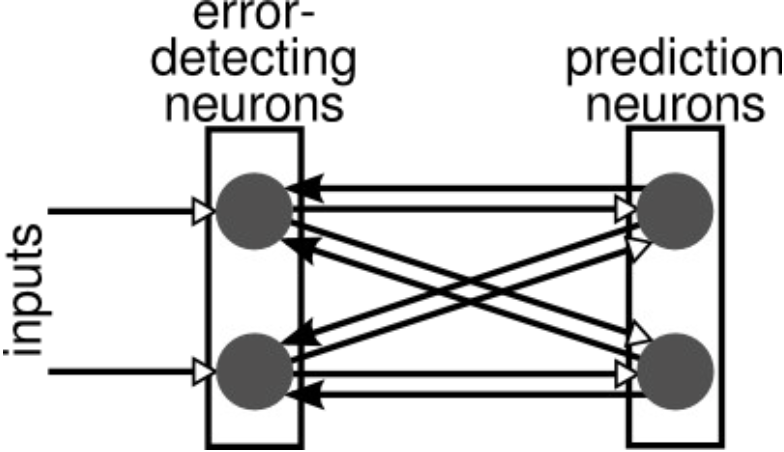
\includegraphics[scale=0.6]{prediction}
			\caption{A graphical representation of a pair of adjacent populations in the PC model. \cite{spratling2014predictive}.}
		\end{figure}
		Predictive coding is commonly used to model information processing in cerebral cortex. It is typically implemented as hierarchical neural networks
		with alternating populations of error-detecting and prediction neurons. Prediction neurons' activity produces a reconstruction of the inputs
		via feedback connections to the preceding error-detecting neurons; error-detecting neurons calculate the residual error between
		the reconstructed and actual inputs \cite{spratling2014predictive}.
		\begin{figure}[H]
  			\centering
			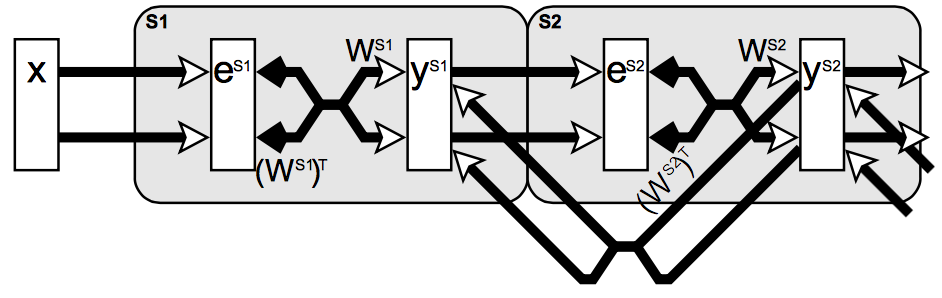
\includegraphics[scale=0.4]{pcbc}
			\caption{A graphical representation of the PC/BC model \cite{spratling2008predictive}.}
			\label{fig:pcbc}
		\end{figure}
		PC/BC is an alternative model that uses direct excitatory feedback from one population of prediction nodes to the preceding one \cite{spratling2008predictive}.
		Activation rules for a PC/BC model as the one in figure~\ref{fig:pcbc} implemented as a hierarchical neural network are as follows:
		
		$$e^{Si} = G(y^{Si-1}) \oslash [\epsilon_2 + (V^{Si})^T y^{Si}]$$
		$$y^{Si} \leftarrow (\epsilon_1 + y^{Si}) \otimes W^{Si}e^{Si} \otimes [1 + \eta G((U^{Si+1}))^T y^{Si+1}]$$
		
		Where:
		\begin{itemize}
			\item $Si$ indicates the stage $i$ of the hierarchical network.
			\item $e^{Si}$ is a $m \times 1$ vector of error-detecting neuron activations.
			\item $y^{Si}$ is a $n \times 1$ vector of prediction neuron activations.
			\item $W^{Si}$, $V^{Si}$, $U^{Si}$ are $n \times m$ matrces of synaptic weights.
			\item $\epsilon_1$, $\epsilon_2$, $\eta$ are parameters.
			\item $G$ is a function that clips values at 1. 
		\end{itemize}
		
		In the first equation, the first term represent the actual input, while the second term represents the reconstructed input from the prediction neurons.
		
		In the second equation, the first term represents the previous value of $y^{Si}$, the second term is the feedforward input from error-detecting neurons to prediction ones, and
		the third term represents the modulation coming from the top-down predicitions of the next stage, if any.
		
		In \cite{spratling2012unsupervised}, Spratling proposes an algorithm to iteratively train the weights of the three matrixes indipendently. For the purpose
		of the project, we are especially interested in tuning the parameter $n$, that is, the number of prediction neurons or, equivalently, the number of
		the possible types of components in an image. That is a value which is in general not known \emph{a priori}, and it is especially suited to be
		the main target of the constructive algorithm. For example, a neuron can be added to the prediction layer and a row can be added to the matrixes
		if the error values stay over a certain value.
		
	\subsection{Constructive Neural Network algorithms}
		Constructive algorithms are used to adjust the structure of a neural network during the learning phase.
		Different approaches are possible: a purely constructive one adds layers, neurons and connections starting from a minimal architecture; pruning
		starts from a complex structure and removes redundant parts; the two approaches can also be combined \cite{parekh2000constructive}.
		
		The advantages of using a constructive algorithm are, among the others:
		\begin{itemize}
			\item It is flexible: the whole space of possible neural network configurations can be explored.
			\item The initial configuration of the model is minimal and straightforward.
			\item Final configurations can be thought as estimating the real complexity of the learned problem.
		\end{itemize}
		
		There exists various constructive algorithms:
		The CC algorithm produces neural networks with multiple hidden layers, with one neuron each that is connected to all other neurons previously added \cite{sharma2010constructive}
		This is not the kind of structure that is needed for the project; so it is not appropriate.
		
		DNC add neurons in a hidden layer until the network achieves an approximation of the desired perfomances.
		Every time a neuron is added, all the weights are retrained. This is effective but at the expence of computational cost. \cite{sharma2010constructive}
		
		OHL-FNN is an extension of DNC that freezes the neural network weights that have been previously trained,
		and that retrains only the weights affected by the insertion \cite{kwok1997objective}.
		
		The last two algorithms can be used in the project's problem by adding a neuron to the prediction layer based on the values
		of the error-detection activations.

\section{Gantt chart}
		\begin{figure}[H]
  			\centering
			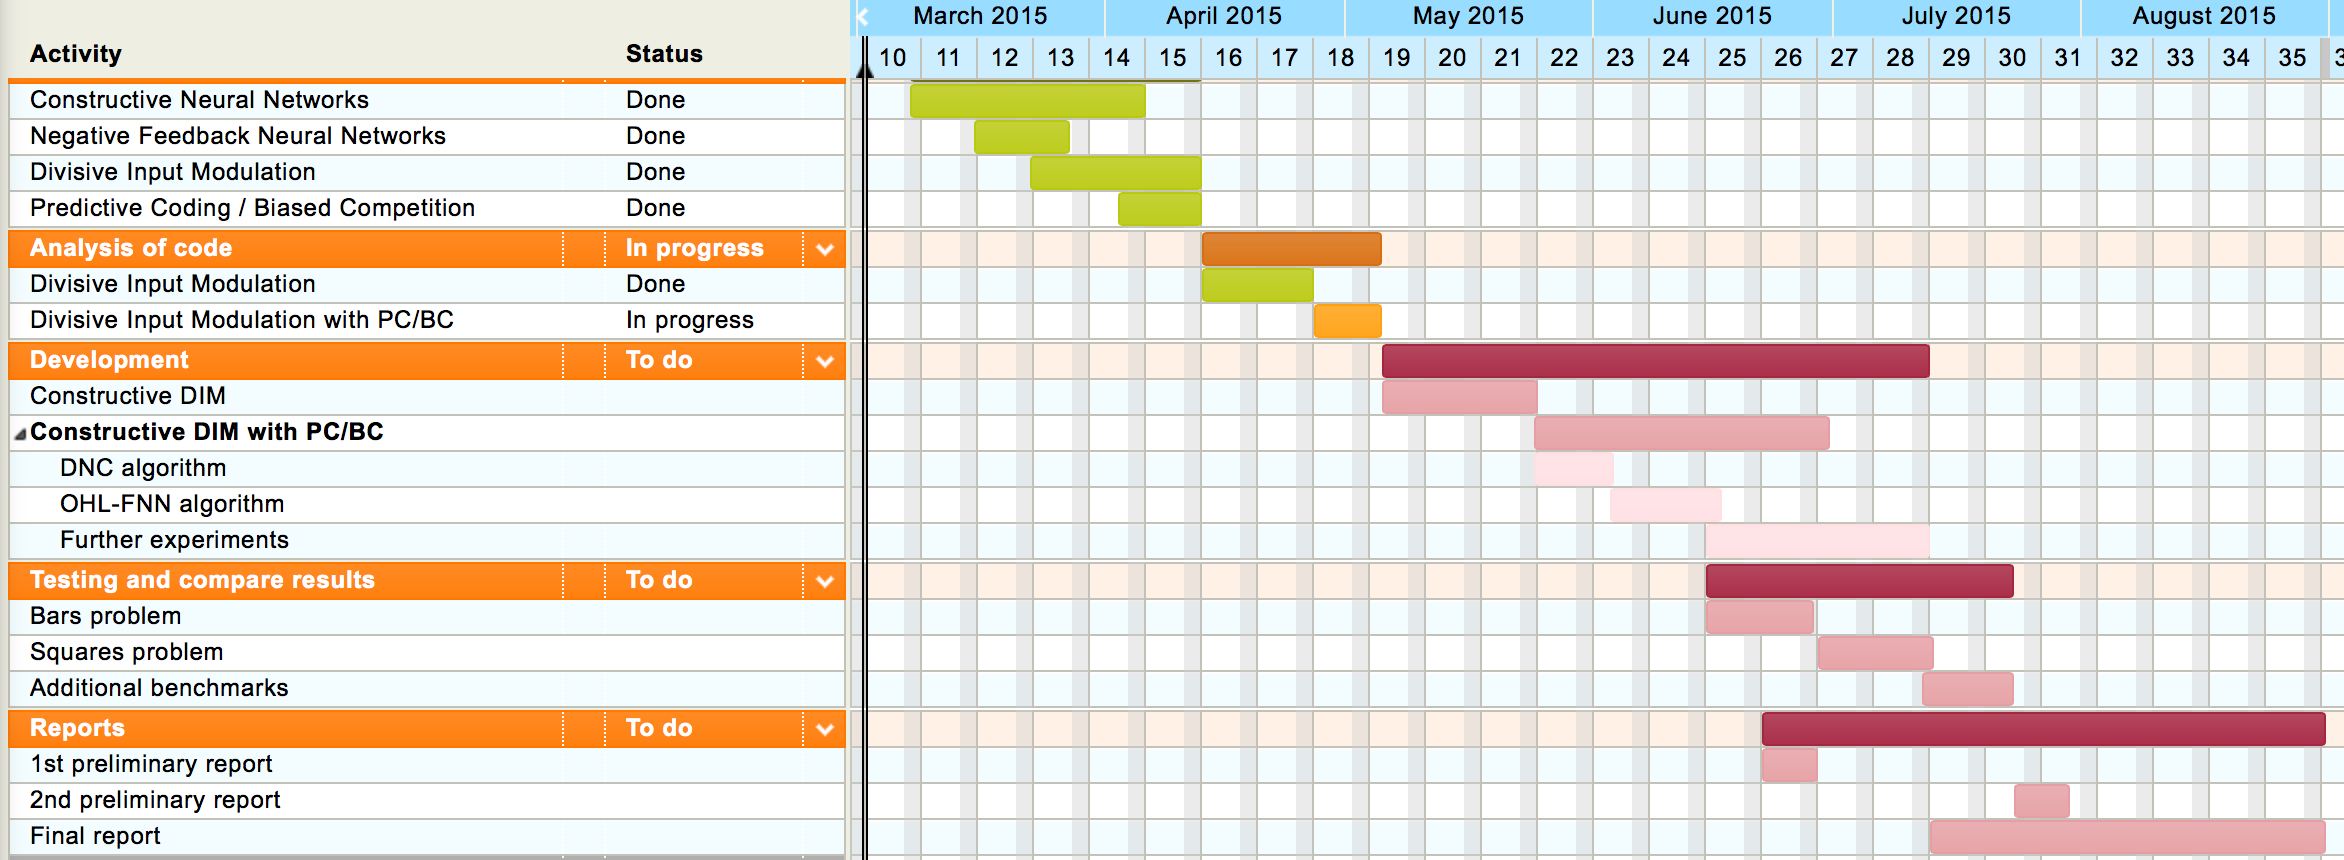
\includegraphics[width=1.1\textwidth]{gantt}
		\end{figure}
		
		
\bibliographystyle{plain}
\bibliography{biblio}

\end{document}